\documentclass[11pt]{article}

\usepackage{paralist}
\usepackage{amsmath}
\usepackage{textcomp}
\usepackage[top=0.8in, bottom=0.8in, left=0.8in, right=0.8in]{geometry}

% Add other packages here %
\usepackage{graphicx}
\usepackage{array}

% Put your group number and names in the author field %
\title{\bf Exercise 1.\\ Implementing a first Application in RePast: A Rabbits Grass Simulation.}
\author{Group \textnumero76: Simon Honigmann, Arthur Gassner}

\begin{document}
\maketitle

\section{Implementation}

\subsection{Assumptions}
% Describe the assumptions of your world model and implementation (e.g. is the grass amount bounded in each cell) %
On top of the directions given in the exercise, our assumptions are the following :\\

\begin{compactenum} 
	\item Only one grass can occupy a tile.
	\item Only one rabbit can occupy each tile.
	\item Grass can grow on a tile already occupied by a rabbit.
	\item If a rabbit is surrounded by other rabbits in all 4 cardinal directions, it simply does not move. The rabbit still has the chance to eat grass or reproduce if possible.
	\item The grid is a square, so only one dimension is required.
\end{compactenum}

\subsection{Implementation Remarks}
% Provide important details about your implementation, such as handling of boundary conditions %
Below are some remarks concerning the way the simulation was implemented :\\

\begin{compactenum}
	\item Eating grass increments the amount of energy of the rabbit by 4, and removes the grass from that tile.
	\item At birth, rabbits have 20 energy.
	\item Each rabbit loses 1 energy per step.
	\item When a rabbit reproduces, it loses 15 energy.
	\item When a rabbit has enough energy to give birth but there are already too many rabbits in the space, then the rabbit does not reproduce. No energy is lost for the unsuccessful attempt to reproduce. 
	\item The number of rabbits cannot be set higher than the total amount of tiles on the grid. Trying to do so informs the user that it cannot be done and the last valid value is used.
	\item Negative user inputs are invalid and interpreted to be 0. 
	\item The growth rate of the grass cannot be set higher than the total amount of tiles on the grid. Trying to set an invalid value creates a pop-up message informing the user of their mistake. The last valid value is maintained. 
	\item The simulation will be scheduled to stop if there are no living rabbits, and either grass has filled the screen or grass growth rate is zero. Then it waits 10 steps before stopping to allow the graphs to appropriately reflect the final state.\\
	
\end{compactenum}

\section{Results}
% In this section, you study and describe how different variables (e.g. birth threshold, grass growth rate etc.) or combinations of variables influence the results. Different experiments with different settings are described below with your observations and analysis
In order to explore the complex and semi-random nature of the population behaviours, several different combinations of values were explored.\\

In the first experiment, we wanted to determine the effect of grid size on the perceived randomness of the population dynamics. Starting with a large grid size, parameters were selected to display a characteristic damped-harmonic-oscillator behaviour. The grid size was reduced to 20\% its original value, and the initial number of rabbits and grass growth rate were reduced to 4\% (20\% squared) to remain proportional to the grid area.\\

In the second experiment, we wanted to explore the behaviour of xxx\\

In the third simulation, a smaller grid size with length 10 and 100 total tiles was used.\\

\subsection{Experiment 1}
\begin{figure}[h]
	\centering
	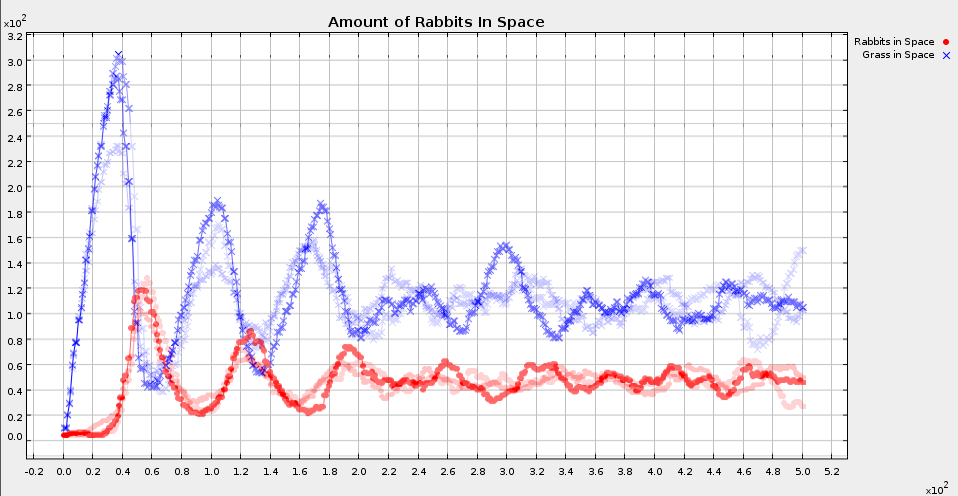
\includegraphics[height=1.5in,width=3.3in]{ex2}
	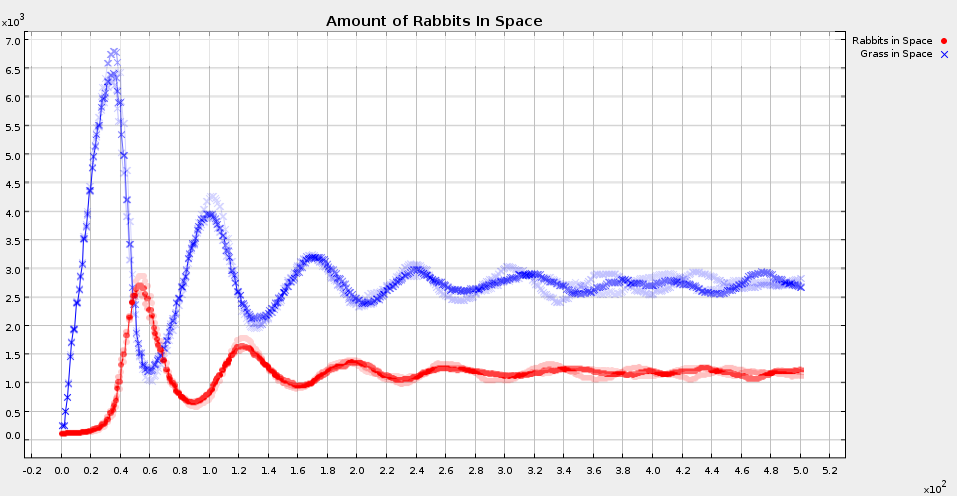
\includegraphics[height=1.5in,width=3.3in]{ex1}
	\caption{Rabbits population (red) and grass population (blue) over three trials using a grid of 400 tiles (left) and 10000 tiles (right). Other parameters are held proportionally constant.}
	\label{figure:1}
\end{figure}
\subsubsection{Setting}

The settings used for the two above simulations are specified here. The settings were untouched for each of the three trials we ran per simulation.\\

\begin{table}[h]
	\centering
	\begin{tabular}{ | c | c | c | } 
		\hline
		\qquad & left side & right side \\ 
		\hline
		Amount Rabbits & 4 & 100 \\ 
		\hline
		Birth Threshold & 20 & 20 \\
		\hline
		Grass Growth Rate & 10 & 250 \\
		\hline
		Grid Size & 20 & 100 \\  
		\hline
	\end{tabular}
	\caption{Table specifying the settings of the two above simulations}
	\label{table:1}
\end{table}

\subsubsection{Observations}
% Elaborate on the observed results %
The large grid size helps eliminate the effect of the random steps on a population's rise or fall. Because the randomness is averaged over such a large number of agents, a near-perfect damped harmonic oscillator can be observed on the population graphs (c.f. right image of Figure 1).\\

A similar looking damped harmonic oscillator can be observed on the left side of the Figure 1., but with much more random noise and more discrepancies in-between each trial.\\

We can also see that the frequency of both near-perfect damped harmonic oscillators are the same. We could hypothesize that scaling grass growth rate, amount of rabbits and grid size the way we did conserves the shape of the population plot.\\

We also notice a phase delay between the rabbit population plot and the grass population plot. This makes sense given that the rabbits need some time to stumble upon the grass and eat it, time during which the grass can grow.\\
\subsection{Experiment 2}
\begin{figure}[h]
	\centering
	%\includegraphics[height=1.5in,width=3.3in]{}
	\caption{TODO}
	\label{figure:2}
\end{figure}
\subsubsection{Setting}

The settings used for the three above simulations are specified here. The only setting changing is the amount of rabbits present on the grid at the beginning of the simulation.\\

\begin{table}[h]
	\centering
	\begin{tabular}{ | c | c | c | c | } 
		\hline
		\qquad & left & middle & right \\
		\hline
		Amount Rabbits & 10 & 100 & 1000\\ 
		\hline
		Birth Threshold & 20 & 20 & 20 \\
		\hline
		Grass Growth Rate & 120 & 120 & 120 \\
		\hline
		Grid Size & 100 & 100 & 100\\  
		\hline
	\end{tabular}
	\caption{Table specifying the settings of the three above simulations}
	\label{table:2}
\end{table}

\subsubsection{Observations}
We can see that, provided that the rabbits manage to survive and reproduce, the amount of rabbits present on the grid at the beginning of the simulation does not influence the steady-state values of the population plots (all other settings being kept the same).\\

Another interesting result is that a phase shift occurs as we change the Amount Rabbits. That is to expect, since the less rabbits initially on the grid, the more time they need to breed and reach the "critical" amount of rabbits where their expansion suddenly accelerates quickly. That time needed by the rabbits to breed is translated on the graph by that phase shift.\\






\end{document}